		Once a card has been isolated from an image and its perspective correctly transformed, the isolated suit symbol in the top-left corner is compared to a set of pre-created symbols using the previously discussed Hit-or-Miss Transform.

		This operation is completed in two stages. First, the suit colour is determined, then the symbol is pattern matched. The suit search space is halved by the suit colour evaluation and also aids detection accuracy by defining pairs of suits as mutually exclusive in the detection. For example, a hearts symbol cannot be miss-classified as a spaces symbol once the colour of the suit is determined.

		\begin{figure}[H]
			\centering
			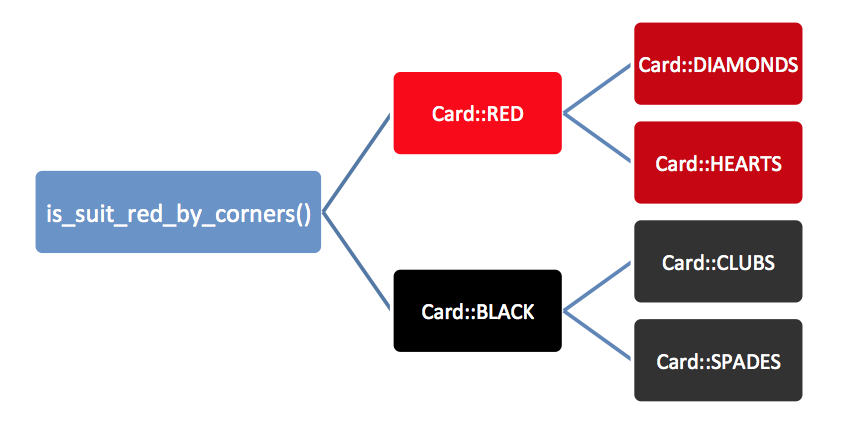
\includegraphics[width=0.95\textwidth]{chris/image38}
			\caption{Flow diagram of suit symbol classification showing mutually exclusive possibilities based on detected colour.}
		\end{figure}

		This decision is shown in the code segment below:

		\begin{lstlisting}

//Do matches using colour info integration
if(card->detected_colour == Card::RED)
{
	matches[DIAMOND] += (int)round(hit_or_miss_score(mat_sym_1c, se_symbols[DIAMOND]) * 100.0F);
	matches[HEART] += (int)round(hit_or_miss_score(mat_sym_1c, se_symbols[HEART]) * 100.0F);
}
else if(card->detected_colour == Card::BLACK)
{
	matches[CLUB] += (int)round(hit_or_miss_score(mat_sym_1c, se_symbols[CLUB]) * 100.0F);
	matches[SPADE] += (int)round(hit_or_miss_score(mat_sym_1c, se_symbols[SPADE]) * 100.0F);
}
else
{
	cout << "Colour has not been detected before find_suit_sym()!" << endl;
	return;
}
		\end{lstlisting}

		The second stage is performed with the Hit-or-Miss Transform applied to the isolated symbol \code{cv::Mat} using each of four pre-created symbol images, shown in Figure~\ref{fig:structelems}, after being resized to the same dimensions.

		\begin{figure}[H]
			\centering
			\begin{subfigure}[b]{0.15\textwidth}
				\centering
				
\includegraphics[width=\textwidth]{chris/image28}
				\caption{}
			\end{subfigure}
			\begin{subfigure}[b]{0.15\textwidth}
				\centering
				
\includegraphics[width=\textwidth]{chris/image29}
				\caption{}
			\end{subfigure}
			\begin{subfigure}[b]{0.15\textwidth}
				\centering
				
\includegraphics[width=\textwidth]{chris/image30}
				\caption{}
			\end{subfigure}
			\begin{subfigure}[b]{0.15\textwidth}
				\centering
				
\includegraphics[width=\textwidth]{chris/image31}
				\caption{}
			\end{subfigure}
			\caption{The four pre-created suit symbol structuring elements.}
			\label{fig:structelems}
		\end{figure}

		Once both of the two applicable coloured structuring element images have been compared, the winning percentage match is then attributed in the structure for that card:

		\begin{lstlisting}

//Find which suit was matched most
if(max(matches[CLUB], matches[DIAMOND], matches[HEART], matches[SPADE]) == matches[CLUB])
{
	cout << "Suit may be CLUBS!" << endl;
	card->detected_suit = Card::CLUBS;  
}
else if(max(matches[CLUB], matches[DIAMOND], matches[HEART], matches[SPADE]) == matches[DIAMOND])
{
	cout << "Suit may be DIAMONDS!" << endl;
	card->detected_suit = Card::DIAMONDS;
}
else if(max(matches[CLUB], matches[DIAMOND], matches[HEART], matches[SPADE]) == matches[HEART])
{
	cout << "Suit may be HEARTS!" << endl;
	card->detected_suit = Card::HEARTS;
}
else if(max(matches[CLUB], matches[DIAMOND], matches[HEART], matches[SPADE]) == matches[SPADE])
{
	cout << "Suit may be SPADES!" << endl;
	card->detected_suit = Card::SPADES;
}
else
{
	cout << "No winner! UNKNOWN SUIT" << endl;
	card->detected_suit = Card::UNKNOWN_SUIT;
}
		\end{lstlisting}

		This matching is shown visually in the figure below in the case of a hearts card:

		\begin{figure}[H]
			\centering
			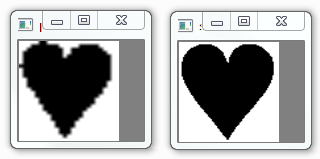
\includegraphics[width=0.6\textwidth]{chris/image32}
			\caption{Isolated and segmented card suit symbol and pre-created template used for comparison.}
		\end{figure}

		In this way the suit symbol is identified as contributes to the classification of the card in question.